%\chapter{Analysis and Design}
\chapter{Analiză și proiectare}
\label{cap:analiza-si-proiectare}

In acest capitol este descris design-ul proiectului si cuprinde: cerintele sistemului, specificatiile cazurilor de utilizare, arhitectura sistemului, comportamentul sistemului, datele utilizate de sistem, dependintele sistemului si algoritmi esentiali si metodele folosite. Descrierea acestora se realizeaza prin asocierea cu diagramelor aferente.

\section{Cerintele sistemului}

Sistemul propus \textit{\thesistitle} reprezinta un software gratis care ofera clientului atat caracteristici specificie unui reverse proxy, cat si modalitati de protectie asemeni unui sistem de prevenire a intruziunilor.
Sistemul este usor de instalat si de utilizat, chiar si de catre utilizatorii neexperimentati, oferindu-le acestora o interfata clara si sugestiva, ce mascheaza logica complicata din spate. In spate, sistemul ofera un reverse proxy ce intercepteaza tot traficul destinat catre un anumit server, de pe una sau mai multe interfete. In procesul de interceptare, acesta implementeaza si cateva modalitati de prevenire a unor tentative de intruziune. Sistemul blocheaza toate ip-urile utilizate frecevent de reteaua Tor in ultima luna si atacurile de SQL injection cu o acuratete de 90\%.

Sistemul trebui sa indeplineasca urmatoarele cerinte \textbf{functionale}:
\begin{enumerate}
	\item Sa realizere conexiunea la un server HTTP/HTTPS si sa redirectioneze traficul primit catre acesta.
	\item Sa intercepteze traficul venit pe o anumita interfata si port prestabilit.
	\item Sa prelucreze request-urile primite de la clineti intr-un format specific clasificatorului de SQL injection.
	\item Sa nu redirectioneze reqesturile clasificate ca si SQL injection.
	\item Sa blocheze conectarea clientilor ce folosesc ip-uri clasificate ca ip-uri de Tor.
	\item Sa permita utilizatorului sa editez si sa vizualizeze lista ip-urilor de Tor.
	\item Sa prezinte in interfata grafica toate interventiile rezlizate asupra traficului(blocari de conexiuni sau de request-uri).
	\item Sa permita utilizatorului sa configureze modul de operare al sistemului.
\end{enumerate}

Sistemul trebuie, de asemenea, să aibă următoarele caracteristici \textbf{non-funcționale}:
\begin{enumerate}
	\item Sa fie usor de instalat si de folosit pentru orice utilizator, oricat de neexperimentat.
	\item Sa poata intercepta traficul de pe orice/oricate interfete disponibile.
	\item Sa poata rula pe orice sistem de operare Windows cu Python2 instalat.
	\item Sa aiba o rata de blocare de 100\% a ip-urilor de pe lista neagra, iar
	in cazul detectiei de SQL injection sa nu aiba detectii false pozitive mai mari 2-3\%
	si o acuratete generala de peste 90\%
\end{enumerate}
\newpage

\section{Specificatiile cazurilor de utilizare}

\subsection{Actori, stakeholders si interese}

Principalii actori si stakeholder-i sunt administratorii de servere, respectiv de baze de date. In implementarea sistemului propus se urmareste satisfacerea nevoilor acestor persoane, oferindule un plus de securitate asupra datelor ce sunt accesate de catre clienti, respectiv impotriva clientilor rau intentionati. Interesele acestor comunitati de utilizatori sunt urmarite pentru a livra un produs care sa ofere aceste protectii intr-o maniera cat de prietenoasa pentru utilizator si cat mai eficienta.

\subsection{Basic flow}

\begin{figure}[h]
	\centering
	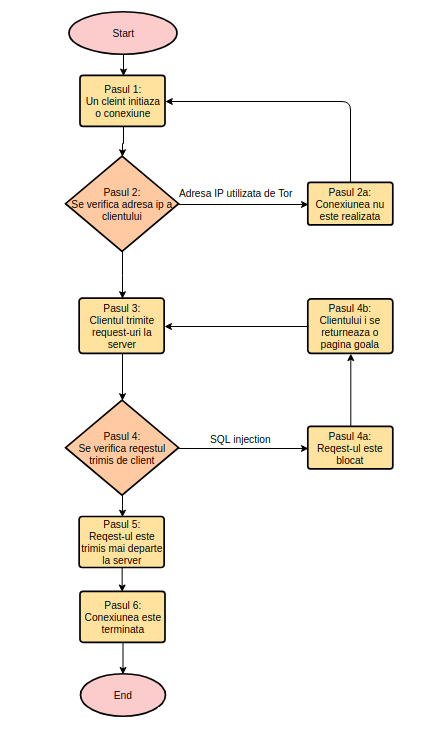
\includegraphics[width=0.4\textwidth]{basicflow.png}
	\caption{Basic flow pentru evenimente}
	\label{fig:basic-flow}
\end{figure}
Figura ~\ref{fig:basic-flow} prezinta cum arata basic flow-ul pentru evenimentele din sistemul propus. \\

Evenimentele sistemului:
\begin{enumerate}
	\item \textbf{Start}: aceste cazuri de utilizare sunt initiate in momentul in care sistemul este plasat intre un server si utilizatorii acestuia.
	\item \textbf{Pasul 1}: un client doreste si initializeze o conexiune la server.
	\item \textbf{Pasul 2}: adresa ip a clientului este verificata ca acesta sa nu fie un utilizator de Tor.
	\item \textbf{Pasul 3}: clientul comunica cu serverul prin reqest-uri individuale.
	\item \textbf{Pasul 4}: reqest-urile sunt verificate ca acestea sa nu fie atacuri de SQL injection.
	\item \textbf{Pasul 5}: request-urile sunt trimise mai departe catre server.
	\item \textbf{Pasul 6}: conexiunea este terminata(de catre client sau server).
	\item \textbf{End}: la sfarsitul unui sir de evenimente, utilizatorul sistemului poate sa vada daca clientul ce a initializat evenimentele a realizat actiuni considerate ca malitioase.
	
	
\end{enumerate}


\subsection{Alternative flow}
Evenimentele alternative in cazurile de utilizare sunt urmatoarele:
\begin{enumerate}
	\item \textbf{Pasul 2a}: in cazul in care un utilizator cu adresa ip de Tor incearca sa realizeze conexiunea la server aceasta este refuzata. 
	\item \textbf{Pasul 4a}: in cazul in care un utilizator incearca sa trimita la server un request ce reprezinta o tentativa de atac SQL injection, acesta este blocat.
	\item \textbf{Pasul 4b}: pentru request-urile blocate ca si SQL injection clientului i se returneaza o pagina goala. 
\end{enumerate}

\newpage


\section{Arhitectura sistemului si modulele principale}

In conformitate cu cerintele sistemului si specificatiile cazurilor de utilizare, sistemul propus este alcatuit din module specifice care sa trateze in mod individual problemele majore ridicate de sistem, printr-o implementare modulara, oferind astfel usurinta implementarii de noi functionalitati.

\begin{figure}[h]
	\centering
	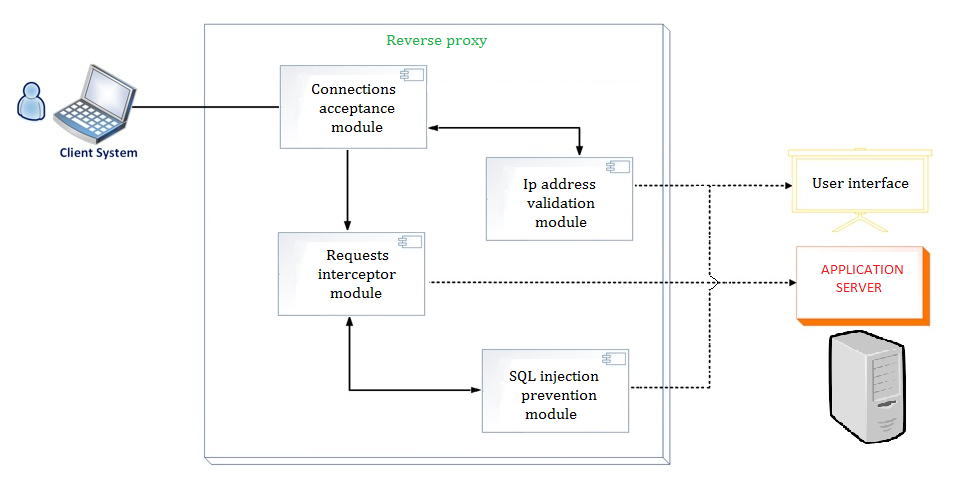
\includegraphics[width=0.8\textwidth]{module.png}
	\caption{Principalele module ale sitemului propus}
	\label{fig:module}
\end{figure}
Figura ~\ref{fig:module} prezinta care sunt pricipalele module ale sistemului propus, precum si interactiunea dintre acestea. \\

\textbf{Client system} si \textbf{application server}.\\

Aceste doua componente reprezinta componetele clasice intre care vin plasat sistemul propus. \textbf{Client system} este reprezentat de orice client doreste sa acceseze baza de date/parte de server a unei aplicatii. \textbf{Application server} reprezinta serverul aplicatie la care se pot conecta clientii pentru a avea acces la un anumit continut. Sistemul propus are rolul de intermediere intre cele doua tipuri de componente, prevenind astfel eventuale tentative de expluatare a unor vulnerabilitati din partea clientului catre server.

%Acest capitol descrie design-ul proiectului și cuprinde, în general: 
%\begin{enumerate}
%  \item ilustrarea arhitecturii generale și detaliate a sistemului implementat, care să evidențieze modulele componente și relațiile dintre acestea
%  \item stările prin care trece sistemul în decursul funcționării sale (diagrame de stare)
%  \item modul de interacțiune dintre module și funcționalitatea acestora ilustrată prin diagrame de secvențe
%  \item descrierea algoritmilor/metodelor pe care se bazează funcționarea sistemului dezvoltat
%  \item descrierea organizării/structurii eventualelor baze de date folosite
%  \item justificarea alegerilor/deciziilor făcute și analiza critică a acestora (avantaje și dezavantaje), prin comparație cu alte alternative posibile
%\end{enumerate}
%
%Ca idee generală, design-ul trebuie să fie prezentat independent de o implementare anume, în general, și de cea a voastră, în particular. De asemenea, descrierea design-ului trebuie să conțină toate elementele și detaliile necesare, astfel încât altcineva decât voi să poate realiza o implementare a lui, fără a fi nevoit să ia decizii arhitecturale sau organizare (adică, de design) și să vă contacteze pentru a-și lămuri anumite aspecte neclare.
%
%Capitolul trebuie organizat pe secțiuni și subsecțiuni astfel descrierea să urmeze un cors logic și ușor de urmărit. 
%
%Ponderea acestui capitol relativ la întreaga lucrare este de 25-35\%.
%
%
%\section{Examples: lists, figures, tables, equations}
%
%Așa arată o listă de elemente nenumerotate:
%\begin{itemize}
%  \item element 1
%  \item element 2
%  \item \dots
%\end{itemize}
%
%
%Așa arată o listă de elemente numerotare:
%\begin{itemize}
%  \item element 1
%  \item element 2
%  \item \dots
%\end{itemize}
%
%
%Așa arată o listă în text: 
%\begin{inparaenum}[(\itshape 1 \upshape)]
%  \item element 1, 
%  \item element 2, 
%  \item \dots
%\end{inparaenum}
%
%\textbf{Atenție}: orice tabel, figura sau ecuație (formulă) trebuie referite \textit{explicit} în text explicit (de genul: în Figura X este ulustrat \dots, în Tabelul Y se poate vedea \dots), pentru că Latex le poate plasa chiar și pe altă pagină decât acolo unde vrem noi să ne referim la ele. Vedeți exemple de mai jos!
%
%Tabelul~\ref{table:example} ilustrează un exemplu de tabel. Un editor on-line de tabele poate fi găsit la \url{http://www.tablesgenerator.com/}. 
%
%\begin{table}[t]
%\centering                          % tabel centrat 
%\begin{tabular}{|c|c|c|c|}          % 4 coloane centrate 
%\hline\hline                        % linie orizontala dubla
%Case & Method\#1 & Method\#2 & Method\#3 \\ [0.5ex]   % inserare tabel
%%heading
%\hline                              % linie orizontal simpla
%1 & 50 & 837 & 970 \\               % corpul tabelului 
%2 & 47 & 877 & 230 \\
%3 & 31 & 25 & 415 \\[1ex]           % [1ex] adds vertical space
%\hline                              
%\end{tabular}
%\caption{Nonlinear Model Results}   % titlul tabelului
%\label{table:example}                % \label{table:nonlin} introduce eticheta folosita pentru referirea tabelului in text; referirea in text se va face cu \ref{table:nonlin}
%\end{table}
%
%În Figura~\ref{fig:exemplu} 
%
%\begin{figure}
%    \centering
%    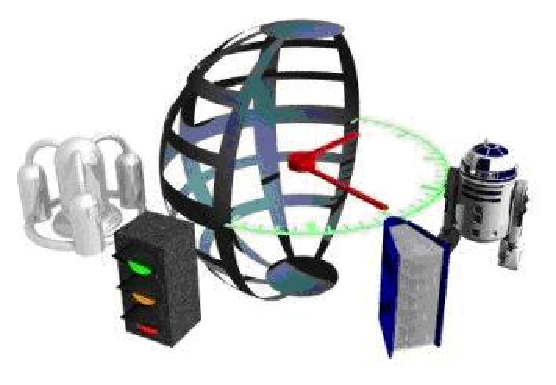
\includegraphics[width=0.5\textwidth]{image}
%    \caption{Numele figurii}
%    \label{fig:exemplu}
%\end{figure}
%
%
%Formula~(\ref{eq:example}) arată modul de calcul al lui $\Delta$:
%\begin{equation} \label{eq:example}
%    \Delta =\sum_{i=1}^N w_i (x_i - \bar{x})^2 .
%\end{equation}
%
%
%Algoritmul~\ref{alg:example} este un exemplu de descriere pseudo-cod a unui algoritm, preluat de la \href{http://en.wikibooks.org/wiki/LaTeX/Algorithms#Typesetting_using_the_algorithm2e_package}{http://en.wikibooks.org/wiki/LaTeX}. El utilizează pachetul \textit{algorithm2e}. Alternativ, puteți utiliza pachetele \textit{algorithmic} sau \textit{program}. 
%
%\begin{algorithm}
% \KwData{this text}
% \KwResult{how to write algorithm with \LaTeX2e }
% initialization\;
% \While{not at end of this document}{
%  read current\;
%  \eIf{understand}{
%   go to next section\;
%   current section becomes this one\;
%   }{
%   go back to the beginning of current section\;
%  }
% }
% \caption{How to write algorithms}
% \label{alg:example}
%\end{algorithm}
